\documentclass{JNUexp}
\courseName{计算机图形学}
\expName{实验 4 2D/3D 变换}
\expDate{2017.11.30}
\className{计科1404}
\studentName{阎覃}
\studentId{1030414414}

\graphicspath{ {images/} }

\usepackage[hidelinks]{hyperref}
\usepackage{amsmath}
\begin{document} 

\section{实验内容}
模拟一个太阳系星球的运转系统:地球环绕太阳转,月球环绕地球转。

\section{实验步骤及运行情况}
%%%%%%%%%%%%%%%%%%%%%%%%%%%%%%%%%%%%%%%%%%%%%%%%%%%%%%%%%
%   1 模拟一个太阳系星球的运转系统:地球环绕太阳转,月球环绕地球转。
%%%%%%%%%%%%%%%%%%%%%%%%%%%%%%%%%%%%%%%%%%%%%%%%%%%%%%%%%
\begin{problem}
    模拟一个太阳系星球的运转系统:地球环绕太阳转,月球环绕地球转。
\end{problem}

\begin{answer}
以下代码是display函数中控制旋转和绘制太阳、地球、月亮的主要代码。

完整程序在本文最后的网址中。

    \begin{lstlisting}[language=C++]
glPushMatrix();                     // 太阳
glRotatef(90, 1, 0, 0);             // 自转
glRotatef(angle, 0, 0, 1);          // 自转
glBindTexture(GL_TEXTURE_2D, imgSun->id);
gluQuadricTexture(imgSun->quad, 1);
gluSphere(imgSun->quad, 1, 30, 30);
glPopMatrix();
glRotatef(angle, 0, -1, 0);         // 公转
glTranslatef(4, 0, 0);              // 公转

glPushMatrix();                     // 地球
glRotatef(90, 1, 0, 0);             // 自转
glRotatef(angle, 0, 0, 1);          // 自转
glBindTexture(GL_TEXTURE_2D, imgEarth->id);
gluQuadricTexture(imgEarth->quad, 1);
gluSphere(imgEarth->quad, 0.3, 30, 30);
glPopMatrix();
glRotatef(angle, 0, -1, 0);         // 公转
glTranslatef(1, 0, 0);              // 公转

glPushMatrix();                     // 月球
glRotatef(90, 1, 0, 0);             // 自转
glRotatef(angle, 0, 0, 1);          // 自转
glBindTexture(GL_TEXTURE_2D, imgMoon->id);
gluQuadricTexture(imgMoon->quad, 1);
gluSphere(imgMoon->quad, 0.15, 30, 30);
glPopMatrix();
    \end{lstlisting}
\end{answer}

\begin{image}
    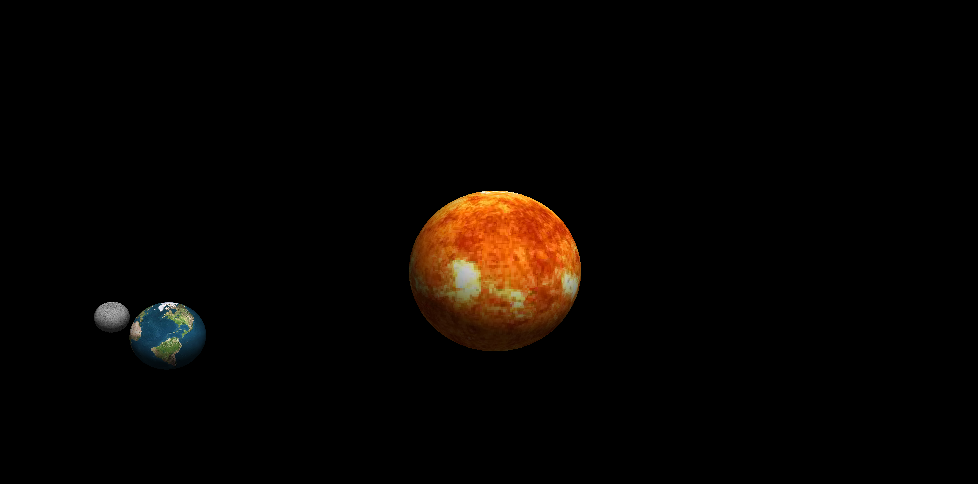
\includegraphics[width=0.7\textwidth]{1}
\end{image}

\newpage
\section{实验体会}
本次试验实现了一个简易的太阳系星球的运转系统,我学会了控制3D变换。为了更逼真我在网上搜索了太阳,地球,月亮的材质图片,使用OpenCV和OpenGL,实现了材质贴图的过程。最后还加入了光线控制。


\vfill

实验报告采用 \LaTeX 排版,完整代码托管至GitHub:\\
\url{https://github.com/Ethan-yt/JNU-CG-exp}

\end{document}